\documentclass[11pt,a4paper]{article}
\usepackage{tikz}
\usetikzlibrary{arrows.meta,positioning}
\usepackage{tabularx}
\usepackage{amsmath,amssymb,amsthm}
\usepackage{geometry}
\geometry{margin=1in}
\usepackage{hyperref}
\usepackage{graphicx}
\usepackage{setspace}
\onehalfspacing

\title{\textbf{Paper D-06: Macroscopic Quantum Systems:\\ A Constraint-Driven Flux Dynamics (CDFD) Perspective}}
\author{Steve Bico Mujjabi, MD\\
\small Independent Researcher\\
\small Founder, Vura Labs\\
\small Kampala, Uganda\\
\small ORCID: 0009-0001-0556-5516}
\date{August 2026}

\begin{document}
\maketitle

% BEGIN SHARED-METHODS POINTER
\noindent\textit{Shared Part IV notation and evidence boundaries are defined in \path{PART_IV_METHODS_AND_CLAIM_BOUNDARY.md}. This paper states only its local observables, comparison, and failure conditions.}
% END SHARED-METHODS POINTER


\begin{abstract}
This paper develops a falsifiable CDFD/AFL model of Macroscopic Quantum Systems. It maps coherent excitation, control signals, and environmental noise to driving flux $\Phi$, decoherence, dissipation, coupling, material boundaries, and measurement to active constraint $C$, shielding, error correction, collective order, and driven control to responsiveness $S$, and preparation history, defects, bath state, and prior measurement to structural memory $M_s$. The target outcome is coherence, transport, phase stability, and response, tested against spectroscopy, coherence measurements, controlled baths, material characterization, and perturbation. The paper treats universality as a shared model architecture rather than an assertion that unlike systems have the same material mechanism. It states the negative result that would make the mapping unnecessary and places the domain claim inside the cumulative CDFD programme and its reproducible runtime boundary.
\end{abstract}

\section{Introduction}

In quantum mechanics, a system exists in a superposition of states until it interacts with its environment. This interaction causes decoherence, collapsing the system into a classical state. In a biological cell, the immense thermal noise and molecular collisions should cause decoherence in femtoseconds.

Yet, experiments motivate active study of high-efficiency excitation transfer and the possible role of transient quantum coherence in photosynthetic complexes. CDFD offers a topological explanation for this survival: biology actively engineers physical constraints to firewall the quantum state from the classical flux.

\section{The Quantum-Biological Adaptive Surface}
We govern the quantum-biological interface using the Adaptive Operating Ratio:
\begin{equation}
    \Psi_s = \left( \frac{\Phi}{C} \right) \cdot S \cdot M_s
\end{equation}

For a specific biological quantum structure (e.g., the FMO complex in green sulfur bacteria):
\begin{itemize}
    \item \textbf{Flux ($\Phi$)}: The chaotic thermal noise, vibrational phonons, and molecular collisions of the surrounding cellular cytoplasm.
    \item \textbf{Constraint ($C$)}: The rigid, highly structured protein scaffold that physically holds the chlorophyll or chromophore molecules in precise alignment.
    \item \textbf{Responsiveness ($S$)}: The ability of the scaffold to dynamically tune its internal vibrations (phonon-assisted coherence) to match the required quantum transitions.
    \item \textbf{Memory ($M_s$)}: The deeply conserved evolutionary architecture of the protein. The exact folding geometry is locked by billions of years of natural selection (high $M_s$), ensuring the precise distances required for quantum tunneling are rigidly maintained.
\end{itemize}

\subsection{Engineering the Coherence Firewall}
To maintain a quantum superposition, the chaotic external thermal flux $\Phi$ must be prevented from interacting with the quantum particles.

The biological system achieves this by constructing a massive structural constraint $C$ via the protein scaffold. The rigid geometry and high memory lock ($M_s$) create a localized topological pocket where the external flux is physically barred from entering. Within this specific microscopic pocket, the local adaptive ratio drops to near zero ($\Psi_s \to 0$).

Because the structured environment can partially shield and tune coupling to the surrounding bath, coherence may persist longer than an unstructured comparison permits. Furthermore, the responsiveness $S$ of the protein scaffold actually utilizes the specific frequencies of the remaining thermal noise to actively "push" the quantum state along the most efficient path (quantum goldilocks effect). Biology does not fight the thermodynamic laws; it expertly manipulates the CDFD constraints to create sheltered sanctuaries where quantum mechanics can operate at room temperature.



\section{Measurement Layer}

% BEGIN PART IV MAJOR CROSS-DOMAIN UPGRADE
\section{Cross-Domain Model Upgrade: Mechanism, Scale, and Tests}

\subsection{Observable Translation}

The paper-specific translation begins with an observable chain rather than a
verbal analogy. For Macroscopic Quantum Systems, the proposed drive is coherent excitation, control signals, and environmental noise.
The active limitation is decoherence, dissipation, coupling, material boundaries, and measurement. Responsiveness is carried by
shielding, error correction, collective order, and driven control, while retained state is represented by
preparation history, defects, bath state, and prior measurement. The outcome to explain is coherence, transport, phase stability, and response.

\begin{table}[htbp]
\centering
\small
\caption{Operational CDFD/AFL map for Paper D-06.}
\begin{tabularx}{\textwidth}{|l|X|X|}
\hline
\textbf{Term} & \textbf{Paper-specific observable meaning} & \textbf{Measurement question} \\
\hline
$\Phi$ & coherent excitation, control signals, and environmental noise & What rate, load, gradient, or demand enters the focal system? \\
\hline
$C$ & decoherence, dissipation, coupling, material boundaries, and measurement & Which measured bottleneck limits transfer, function, or recovery? \\
\hline
$S$ & shielding, error correction, collective order, and driven control & Which process changes effective capacity or reroutes the load? \\
\hline
$M_s$ & preparation history, defects, bath state, and prior measurement & Which retained state makes equal present loads produce different futures? \\
\hline
$Y$ & coherence, transport, phase stability, and response & Which outcome is predicted out of sample, with uncertainty? \\
\hline
\end{tabularx}
\end{table}

\begin{figure}[htbp]
\centering
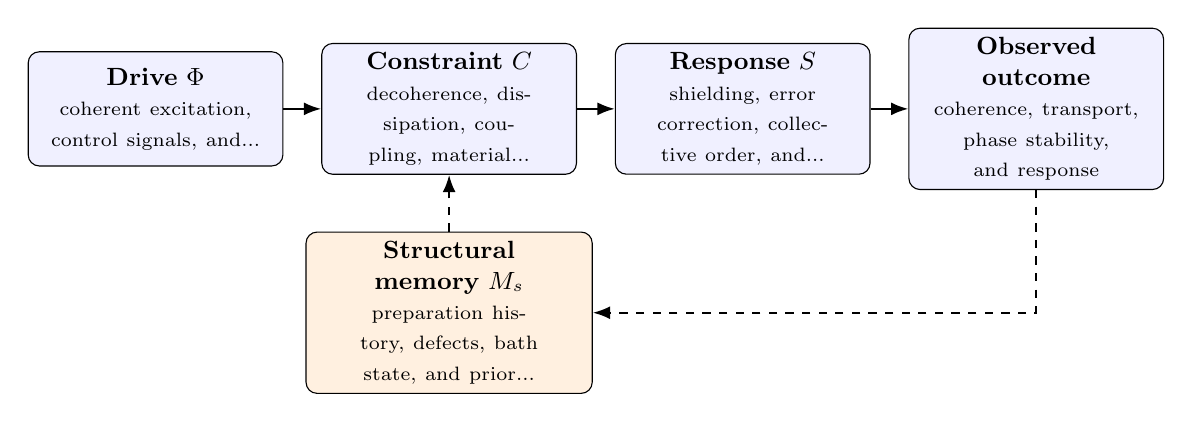
\begin{tikzpicture}[
    node distance=0.48cm,
    every node/.style={font=\small},
    box/.style={draw, rounded corners, align=center, minimum height=1.45cm, text width=3.0cm, fill=blue!6},
    memory/.style={draw, rounded corners, align=center, minimum height=1.25cm, text width=3.4cm, fill=orange!12},
    flow/.style={-{Latex[length=2.2mm]}, thick},
    feedback/.style={-{Latex[length=2.2mm]}, thick, dashed}
]
\node[box] (drive) {\textbf{Drive $\Phi$}\\\scriptsize coherent excitation, control signals, and...};
\node[box, right=of drive] (constraint) {\textbf{Constraint $C$}\\\scriptsize decoherence, dissipation, coupling, material...};
\node[box, right=of constraint] (response) {\textbf{Response $S$}\\\scriptsize shielding, error correction, collective order, and...};
\node[box, right=of response] (outcome) {\textbf{Observed outcome}\\\scriptsize coherence, transport, phase stability, and response};
\node[memory, below=0.72cm of constraint] (memory) {\textbf{Structural memory $M_s$}\\\scriptsize preparation history, defects, bath state, and prior...};
\draw[flow] (drive) -- (constraint);
\draw[flow] (constraint) -- (response);
\draw[flow] (response) -- (outcome);
\draw[feedback] (outcome.south) |- (memory.east);
\draw[feedback] (memory.north) -- (constraint.south);
\end{tikzpicture}
\caption{Paper D-06 observable CDFD/AFL architecture for Macroscopic Quantum Systems. Solid arrows give the proposed forward chain; dashed arrows make history-dependent feedback explicit.}
\label{fig:d06-architecture}
\end{figure}

\subsection{Paper-Specific Causal Hypothesis}

For this paper, the hypothesized causal sequence is specific. A change in
coherent excitation, control signals, and environmental noise arrives faster than shielding, error correction, collective order, and driven control can compensate.
This raises or redistributes decoherence, dissipation, coupling, material boundaries, and measurement. If the load persists,
the retained state encoded by preparation history, defects, bath state, and prior measurement changes the next response, so a later event of equal
magnitude can produce a different trajectory in coherence, transport, phase stability, and response. The
scientific task is to estimate that sequence against the best ordinary model of
the domain, not merely to redescribe the outcome after it occurs.

\subsection{Cross-Scale Translation Without Mechanistic Erasure}

For the domain applications family, the cross-domain translation is a disciplined test across systems with very different material mechanisms. A valid mapping preserves the baseline science of the domain, declares the scale of every variable, and earns its place through a discriminating prediction rather than resemblance alone. \cite{Holling1973,Turing1952,Shannon1948,BakTangWiesenfeld1987}
The required scale declaration for this paper is femtoseconds to device lifetimes; excitations to macroscopic assemblies. At short
scales, the key question is whether the incoming drive is transmitted,
buffered, or diverted. At intermediate scales, response changes effective
capacity and network exposure. At long scales, retained structure can alter the
state space itself. A result is genuinely cross-scale only when the aggregation
rule is stated and the same conclusion is not an artifact of averaging.

\subsection{Evidence Ladder and Discriminating Tests}

\begin{table}[htbp]
\centering
\small
\caption{Evidence ladder for Paper D-06. Each rung can fail independently.}
\begin{tabularx}{\textwidth}{|p{0.17\textwidth}|X|X|}
\hline
\textbf{Test} & \textbf{Design} & \textbf{Discriminating result} \\
\hline
Proxy audit & Measure spectroscopy, coherence measurements, controlled baths, material characterization, and perturbation and preregister how each record maps to $\Phi$, $C$, $S$, $M_s$, and $Y$. & The mapping fails if proxies are non-identifiable, circular, or change meaning across cases. \\
\hline
Load ramp & Apply or observe a calibrated increase in environmental coupling or disorder while estimating the dominant constraint and response time. & A threshold claim requires a reproducible nonlinear change and uncertainty bounds, not a visually chosen breakpoint. \\
\hline
Recovery and memory & Match present load across units with different histories, then compare recovery paths. & The memory claim requires history-dependent divergence after current conditions are controlled. \\
\hline
Model comparison & Compare the baseline domain model with and without the CDFD/AFL state variables using held-out data. & The paper's stated falsifier is: CDFD adds no measurable prediction beyond open-quantum-system theory. \\
\hline
\end{tabularx}
\end{table}

\subsection{Research Programme and Boundary Conditions}

The immediate research programme has four steps. First, construct a documented
dataset from spectroscopy, coherence measurements, controlled baths, material characterization, and perturbation and retain raw units before normalization.
Second, fit a baseline domain model and report its calibration and out-of-sample
error. Third, add the smallest identifiable CDFD/AFL state extension and test
whether it improves prediction of coherence, transport, phase stability, and response. Fourth, repeat the
analysis across the declared scale range and publish negative cases as part of
the cross-domain translation audit.

% END PART IV MAJOR CROSS-DOMAIN UPGRADE

\section{Conclusion}
Macroscopic and biological quantum systems provide a stringent boundary test for CDFD. The useful claim is limited: structured environments may alter coupling, transport, and coherence lifetimes, and the CDFD variables must add a discriminating prediction beyond open-quantum-system theory.
\section*{Conflict of Interest} The author declares no conflict of interest.
\section*{Data Availability}
Part-specific runtime diagnostics are under each Part's \path{outputs/} directory.

Release-wide code: \path{Part_E_Synthesis/supplementary/}.

Generated summaries: \path{Part_E_Synthesis/outputs/}.

Figures: \path{Part_E_Synthesis/figures/}.


\section{Reference Layer}
\bibliographystyle{plain}
\bibliography{universal_afl_references}
\end{document}
